%%%%%%%%%%%%%%%%%%%%%%%%%%%%%%%%%%%%%%%%%%%%%%%%%%%%%%%%%%%%%%%
% Contents : The data management chapter
% $Id : grisbi-manuel-datamanagement.tex, v 0.8.9 2012/04/27 Jean-Luc Duflot
% $Id : grisbi-manuel-datamanagement.tex, v 1.0 2014/02/12 Jean-Luc Duflot
%%%%%%%%%%%%%%%%%%%%%%%%%%%%%%%%%%%%%%%%%%%%%%%%%%%%%%%%%%%%%%%%%

\chapter{Gestion des données\label{datamanagement}}


Les données que vous avez entrées dans Grisbi et les traitements que vous en avez faits sont en nombre important ; de ce fait ils ne doivent en aucun cas être perdus, et leur quantité ne doit pas être un obstacle à leur bonne gestion. Grisbi propose donc trois outils pour faire face à ces problématiques : \menu{Gestion des fichiers de comptes}, \menu{Sauvegardes} et \menu{Archives}.


\section{Gestion des fichiers de comptes\label{datamanagement-files}}


Vous pouvez définir les options de gestion suivantes :

\begin{itemize}
	\item le chargement automatique du dernier fichier consulté ;
	\item l'enregistrement automatique lors de la fermeture ;
	\item le \indexword{forçage de l'enregistrement}\index{enregistrement !forçage} des fichiers verrouillés ;
	\item le \indexword{chiffrement du fichier de comptes}\index{fichier de comptes !chiffrement}\index{chiffrement !fichier de comptes} ;
	\item la \indexword{\gls{compression}} du fichier de comptes\index{fichier de comptes !compression}\index{compression !fichier de comptes} ;
	\item la mémorisation des derniers fichiers ouverts.
\end{itemize}

Toutes ces options sont explicitées en détail et peuvent être configurées dans le menu \menu{Édition - Préférences} (voir le paragraphe \vref{setup-general-files-manage}, \menu{Gestion des fichiers de comptes}).


\section{Sauvegardes\label{datamanagement-backup}}


D'une manière générale, quelles que soient les données que vous possédez dans le disque dur de votre ordinateur, vous devez impérativement en faire des sauvegardes, pour la simple raison que \emph{tout système de stockage de données a une durée de vie limitée}. Faire des sauvegardes a pour but de limiter les risques de pertes de données. 

Grisbi vous permet de faire des sauvegardes automatiques de votre fichier de comptes. Ces sauvegardes devraient être stockées dans un répertoire spécial ou une \gls{partition} spéciale du disque de votre ordinateur, avec les sauvegardes de toutes vos autres données, ce qui vous permettrait alors de sauvegarder facilement ce répertoire ou cette partition, de préférence sur des supports de type différents, indépendants de l'ordinateur, et mis en lieu sûr.

% espace avant Attention ou Note  : 5 mm
\vspacepdf{5mm}
\textbf{Note} : vous êtes maintenant prévenu(e), prenez ces conseils au sérieux : ne prenez pas de risques avec vos données, cela peut vous éviter bien des déboires\ldots
% espace après Attention ou Note  : 5 mm
\vspacepdf{5mm}

Grisbi peut enregistrer automatiquement, dans un répertoire à définir, soit un fichier de sauvegarde unique qui est remplacé régulièrement, soit des fichiers de sauvegarde qui s'accumulent dans ce répertoire.

Les fichiers de sauvegarde ont un nom de la forme \file{nom\_du\_fichier\_AAAAMMJJTHHMMSS.gsb}, où \emph{nom\_du\_fichier} est le nom de votre fichier de comptes, \emph{AAAAMMJJ} est la date en année-mois-jours, \emph{T} est un séparateur, et \emph{HHMMSS} est l'heure en heures-minutes-secondes. Ce format est basé sur le format international de date ISO 8601, ce qui permet, entre autres, le classement automatique dans l'ordre alphanumérique et chronologique dans votre répertoire de sauvegarde.

%espace pour changement de thème
\vspacepdf{5mm}
 Grisbi vous propose les options de sauvegarde suivantes :

\begin{itemize}
	\item la création d'un fichier de sauvegarde unique, sinon les fichiers de sauvegarde s'ajoutent dans  leur répertoire ;
	\item la \indexword{\gls{compression} du fichier de sauvegarde}\index{fichier de sauvegarde !compression}\index{compression !fichier de sauvegarde}, pour occuper moins d'espace disque ;
	\item la sauvegarde après l'ouverture du fichier de comptes ; 
	\item la sauvegarde avant l'enregistrement du fichier de comptes ; 
	\item le réglage de l'intervalle entre deux sauvegardes, en minutes ;
	\item la définition du \indexword{répertoire de sauvegarde}\index{répertoire de sauvegarde}\index{fichier de sauvegarde !répertoire}.
\end{itemize}

%espace pour changement de thème
\vspacepdf{5mm}
Toutes ces options sont décrites en détail et peuvent être configurées dans le menu \menu{Édition - Préférences} (voir le paragraphe \vref{setup-general-files-backup}, \menu{Sauvegardes}).


\section{Archives\label{datamanagement-history}}


Une archive est une sorte de \og mise entre parenthèses \fg{} d'une partie des opérations de tous les comptes de votre fichier de comptes. Les opérations à l'intérieur d'une archive ne sont plus affichées et ne peuvent plus faire l'objet de traitements, mais elles sont toujours conservées dans ce fichier. Vous pouvez toujours et à tout moment désarchiver une archive existante pour en afficher les opérations et l'inclure dans un traitement. 

Lorsque vous utilisez Grisbi, vous entrez des opérations dans vos différents comptes. Ces opérations sont toutes enregistrées dans la mémoire et sur le disque dur de l'ordinateur, et une petite partie est affichée sur l'écran. L'affichage et le traitement des opérations consomme donc de la mémoire et du temps de microprocesseur.

Au fur et à mesure que le temps passe, il y a de plus en plus d'opérations enregistrées, donc leur affichage et leurs traitements demandent de plus en plus d'espace mémoire et de temps de microprocesseur. Votre ordinateur devient donc de plus en plus lent, mais évidemment, cela dépend toujours de ses propres caractéristiques.

Pour limiter cette perte de performances dans l'affichage et le traitement, en particulier dans l'établissement d'états ou dans la recherche d'informations, Grisbi vous propose de choisir une partie des opérations et de les mettre dans une archive, c'est-à-dire de les mettre à part pour leur éviter d'être concernées par de futurs affichages ou traitements.  

La mise en archive peut être manuelle ou automatisée. Grisbi considère qu'au-delà de trois mille opérations{\valeur} dans un compte, les traitements deviennent trop lents, donc d'une part il vous avertit si vous dépassez ce nombre d'opérations et vous propose d'en archiver manuellement une partie, d'autre part il peut vous proposer d'archiver ces  trois mille opérations en lançant automatiquement un assistant.

Que vous fassiez un archivage manuellement ou avec l'assistant, le processus de comptage est ensuite remis à zéro et Grisbi vous proposera de nouveau la même chose après trois mille opérations supplémentaires.


\subsection{Archives dans la liste des opérations\label{datamanagement-history-list}}

L'\indexword{affichage d'une archive}\index{archive !affichage} apparaît tout en haut de la liste des opérations \emph{de chaque compte}, sous la forme d'une ligne d'opération sur fond vert{\couleur}, indiquant sa date de création, son nom et ses paramètres de création (dates, exercice ou état), ainsi que \ifIllustration le \indexword{nombre d'opérations archivées}\index{archive !nombre d'opérations} \emph{pour le compte affiché}, et le \indexword{nombre total d'opérations}\index{opération !nombre total} dans votre fichier de comptes\refimage{datamanagement-history-line-img}.

% image centrée
\begin{figure}[htbp]
\begin{center}
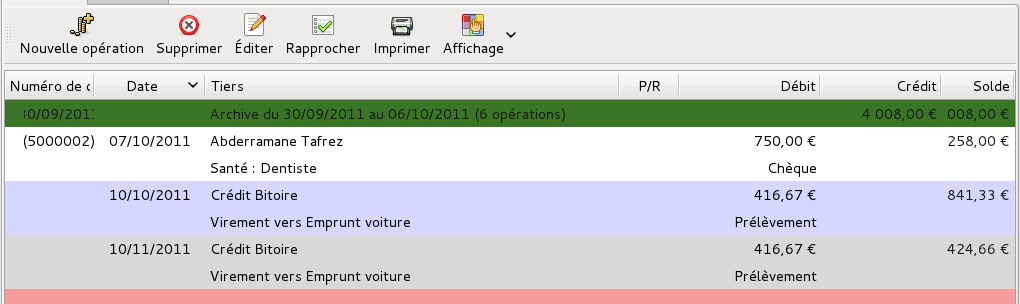
\includegraphics[scale=0.5]{image/screenshot/datamanagement_history_line}
\end{center}
\caption{Ligne d'une archive}
\label{datamanagement-history-line-img}
\end{figure}
% image centrée
\else le \indexword{nombre d'opérations archivées}\index{archive !nombre d'opérations} \emph{pour le compte affiché}, et le \indexword{nombre total d'opérations}\index{opération !nombre total} dans votre fichier de comptes.
\fi

Vous pouvez afficher ou masquer toutes les lignes d'archives dans la liste des opérations de tous les comptes en sélectionnant le menu \menu{Affichage - Montrer les lignes d'archives}, ou en cliquant sur l'outil \menu{Affichage} de la barre d'outils, puis en sélectionnant \menu{Montrer les lignes d'archives} dans sa liste déroulante.

Si vous voulez consulter les opérations à l'intérieur d'une archive, vous pouvez ouvrir cette archive en double-cliquant sur sa ligne : après validation dans la fenêtre qui apparaît, les opérations sont affichées dans la liste. 

\textbf{Note} : il ne s'agit que d'une ouverture de l'archive pour affichage, et en aucun cas cette archive n'est supprimée. À la prochaine utilisation de Grisbi, la ligne verte de l'archive réapparaîtra en haut de la liste de chaque compte. Pour une véritable suppression de l'archive, voir la section \vref{datamanagement-history-remove}, \menu{Suppression d'une archive}.


\subsection{Création d'une archive\label{datamanagement-history-new}}

Pour créer une archive, procédez comme suit :

\begin{enumerate}
	\item dans la barre de menus, sélectionnez \menu{Fichier - Créer une archive} : la fenêtre de l'assistant de création d'archive s'affiche ; validez par le bouton \menu{Suivant} ;
	\item dans la fenêtre suivante, vous pouvez choisir le mode de sélection des opérations à \ifIllustration archiver\refimage{datamanagement-history-create-img} :
	% image centrée
	\begin{figure}[htbp]
	\begin{center}
	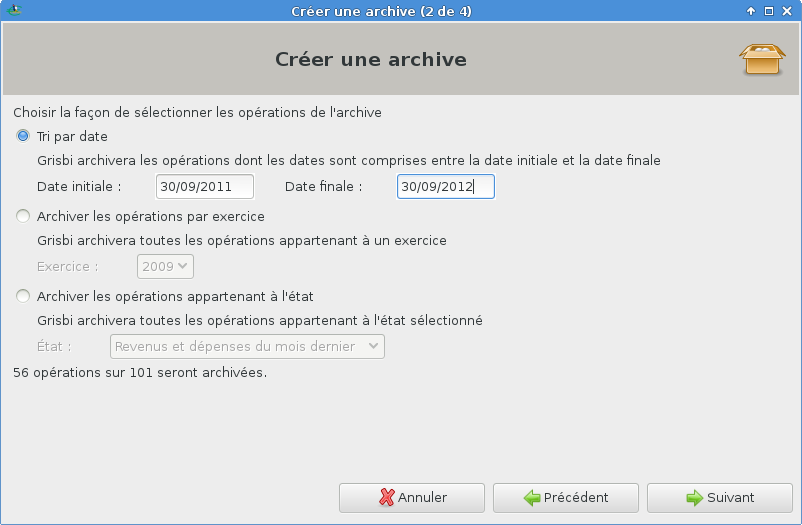
\includegraphics[scale=0.5]{image/screenshot/datamanagement_history_create}
	\end{center}
	\caption{Création d'une archive}
	\label{datamanagement-history-create-img}
	\end{figure}
	% image centrée
	\else archiver :
	\fi
	
		\begin{itemize}
			\item \menu{Tri par date} : saisissez les \menu{Date initiale} et \menu{Date finale} dans les champs adéquats,
			\item \menu{Archiver les opérations par exercice} : sélectionnez un exercice disponible dans la liste déroulante,
			\item \menu{Archiver les opérations appartenant à l'état} : sélectionnez un état disponible dans la liste déroulante ;
% saut de ligne pour indentation correcte de la note dans la liste

			\textbf{Note} : la dernière ligne dans la fenêtre indique soit une erreur de saisie de ces paramètres, soit le nombre d'opérations qui seront archivées et le nombre total d'opérations de votre fichier de comptes.  
		\end{itemize}
	\item validez par le bouton \menu{Suivant} ;
	\item dans la fenêtre suivante, saisissez le nom que vous voulez pour cette archive ; validez par le bouton \menu{Appliquer} ;
	\item la dernière fenêtre vous informe que l'archive a été créée, et affiche le \indexword{nombre d'opérations archivées}\index{archive !nombre d'opérations} et le nombre total d'opérations de votre fichier de comptes, \emph{tous comptes confondus} ; validez par le bouton \menu{Précédent} pour créer une autre archive, sinon par le bouton \menu{Fermer}.
\end{enumerate}

\textbf{Note} :  au cas où Grisbi serait devenu plus lent après avoir créé une archive, vous pouvez le configurer pour ne pas charger les opérations rapprochées (R) au démarrage, afin d'augmenter sa rapidité (voir la section \ref{transactions-functions}, \menu{Barre d'outils}).

% espace après Attention ou Note  : 5 mm
\vspacepdf{5mm}
L'archive apparaît alors tout en haut de la liste des opérations \emph{de chaque compte} (voir la section \vref{datamanagement-history-list}, \menu{Archives dans la liste des opérations}).


\subsection{Avertissement de création et création automatique d'archives\label{datamanagement-history-auto}}

Lorsqu'un certain nombre d'opérations enregistrées est atteint, Grisbi peut d'une part vous avertir que cette quantité d'opérations n'a pas été encore archivée, d'autre part lancer automatiquement la création d'une d'archive  (voir le paragraphe \vref{setup-general-archives-create}, \menu{Avertissement et création automatique}).

En cliquant sur la case libellée \menu{Créer automatiquement une archive si nécessaire}, vous validez la fonction d'archivage automatique.

Avec le libellé \menu{Avertir si plus de \ldots{ } opérations ne sont pas archivées}, vous pouvez définir ce nombre d'opérations. La valeur par défaut est 3000.


\subsection{Paramètres d'une archive\label{datamanagement-history-parameters}}

Vous pouvez consulter les paramètres qui ont été définis pendant la création d'une archive, dans le menu
\menu{Édition - Préférences - Archives}. Pour cela, voir la section \vref{setup-general-archives-existing}, \menu{Archives existantes}.


\subsection{Modification d'une archive\label{datamanagement-history-modify}}

Vous pouvez, uniquement, \indexword{modifier le nom d'une archive}\index{archive !modification} dans le menu \menu{Édition - Préférences}. Pour cela, voir le paragraphe \vref{setup-general-archives-remove}, \menu{Modifier l'archive}.


\subsection{Suppression d'une archive\label{datamanagement-history-remove}}

Vous pouvez \indexword{supprimer une archive}\index{archive !suppression} existante, dans le menu \menu{Édition - Préférences}. Il y a deux fonctions de suppression distinctes : la suppression d'une archive tout en \emph{conservant} ses opérations, et la suppression d'une archive tout en \emph{supprimant} toutes ses opérations. Pour cela, voir le paragraphe \vref{setup-general-archives-remove}, \menu{Modifier l'archive}. 


\subsection{Export d'une archive\label{datamanagement-history-export}}

Exporter une archive permet de créer un fichier contenant l'archive, afin de la stocker, ou de l'utiliser dans un autre fichier de comptes de Grisbi ou dans une autre application de comptabilité. L'exportation ne peut se faire qu'à travers les formats de fichiers \indexword{\gls{GSB}}\index{gsb}, \indexword{\gls{QIF}}\index{qif} ou \indexword{\gls{CSV}}\index{csv}.

% espace avant Attention ou Note  : 5 mm
\vspacepdf{5mm}
\strong{Attention} : les formats de fichiers QIF et CSV ne supportent pas les devises, et toutes les opérations seront converties dans la devise de leur compte respectif.
% espace après Attention ou Note  : 5 mm
\vspacepdf{5mm}

Pour exporter une archive, procédez comme suit :

\begin{enumerate}
	\item dans la barre de menus, sélectionnez \menu{Fichier - Exporter une archive vers un fichier GSB, QIF ou CSV... } : la fenêtre de l'assistant d'exportation d'archive s'affiche ; validez par le bouton \menu{Suivant} ;
	\item un tableau affiche la liste des archives existantes avec leur nom et, selon le cas, leurs dates initiale et finale, leur exercice ou le nom de l'état ; sélectionnez l'archive à exporter en cochant la case dans sa ligne ; validez par le bouton \menu{Suivant} ;
	\item une fenêtre de gestionnaire de fichiers s'affiche ; modifiez éventuellement le nom du fichier sous lequel l'archive sera exportée, le dossier où elle sera enregistrée et le format du fichier d'exportation ; validez par le bouton \menu{Suivant} ;
	\item la dernière fenêtre vous informe que l'archive a été exportée ; validez par le bouton \menu{Fermer}.
\end{enumerate}









